\chapter{Methodology} \label{chap:methodology}
This chapter will present a multi-level model design flow for the integration of heterogeneous applications and their deployment them to the edge on embedded low power devices like NVIDIA Jetson TX2.


\section{A ROS based robotic system}
The choice of the most suitable integration platform is one of the main problems to be faced when integrating heterogeneous applications such as robotic applications. This choice will have implications on performance and communication on the whole system. Furthermore it will be a key factor during the design phase of the entire architecture.
After an accurate comparison among all available robotics platforms, for the purpose of our specific application we decided to use ROS \cite{ROS} in favour of its standard on communication among other applications.

\subsection{Architecture at L1}
At this architecture level we put the whole system on a single Intel x86 powered machine that we will conventionally call \textit{host}. The technical specification of  the host are shown in table ... %TODO table with tech specs

This is the simplest and the most common architecture used by robotics researches. As we can see in figure \ref{fig:l1arch}, we have two main ROS nodes that communicate between them following the ROS standard. Specifically speaking, in this case we have both ORB-SLAM2 and VOVD running as ROS nodes to perform a mobile robot navigation task.

\begin{figure}
	\centering
	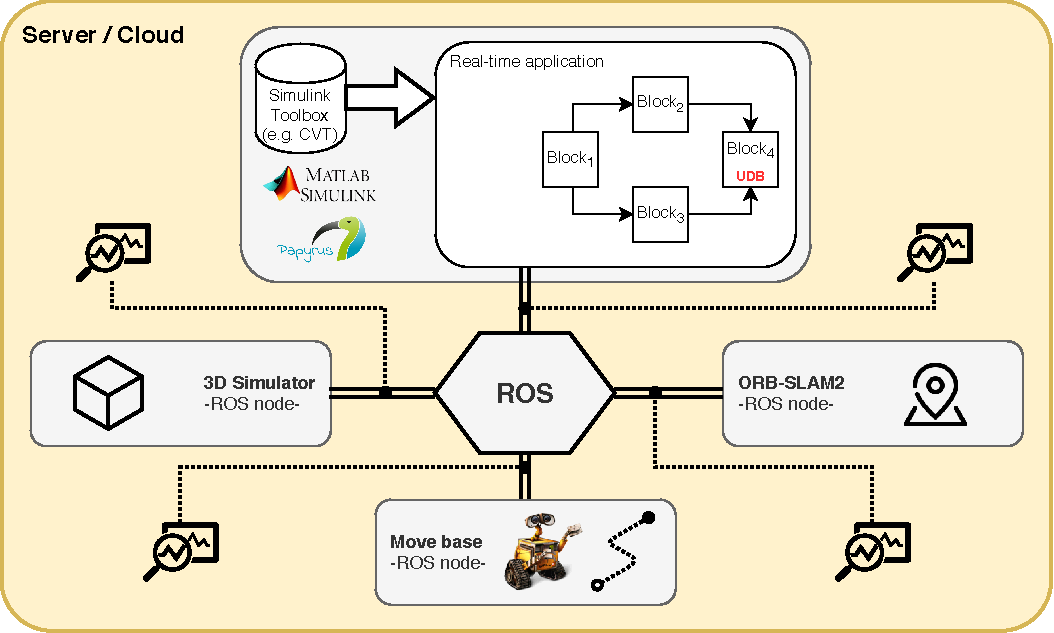
\includegraphics[width=\textwidth]{images/L1_arch}
	\caption{L1 architecture}
	\label{fig:l1arch}
\end{figure}

After the installation of ROS Melodic Morenia \cite{rosmelodic} on our host pc, the first step to achieve this goal has been porting the VOVD \cite{VOVD} application from ROS Kinetic version, with which it was developed, so that the application can be compatible with the our current installed version of ROS. This task required a redefinition of some functions related to the ROS \textit{tf2} package \cite{tfros} due to the deprecation of the \textit{tf} package functions previously used.
ORB-SLAM2 comes already provided with the necessaries functions to run in a ROS environment, so no others operations have been required to complete our first level architecture.

\subsection{Architecture at L2} %TODO Work in progress
The next step require the split of our system ... host - device 


\subsection{Architecture at L3}	%TODO questo non lo abbiamo fatto ...
host - device - robot ...




\section{Deployment from the cloud to the edge}
% How to prepare an application for edge computing in Kubeedge?


\subsection{ORB-SLAM2 at the edge}


\subsection{VOVD at the edge}


\section{The whole system on Kubeedge}



\section{Discussion}



\clearpage
\thispagestyle{empty}